\section{Additional Method Details}

\subsection{Model training}

In this section, we discuss the training setup for \method experiment. 

\textbf{The workers and the batch size.} We use 20 environment workers per GPU. Since we use 4 GPUs in parallel, there are 80 environment workers in total. The micro batch size is 1 and we accumulate the gradient for 10 micro batches on the 4 GPUs which makes the effective batch size 40.

\textbf{RL algorithm.} We use PPO \cite{schulman2017proximal} to train the model with $\gamma=0.99$, $\tau=0.95$, entropy coefficient of 0.1 and value loss coefficient of 0.5.

\textbf{Optimizer.} We use Adam \cite{kingma2014adam} optimizer to learn the parameters.

\textbf{Learning rate schedule.} We use learning rate warm up in the first 100,000 environment interactions. The learning rate starts with $LR_0=2e-7$ and reaches $LR=2e-4$ at the end of the warm up. Cosine decay \cite{loshchilov2017sgdr} is used after the warm-up to decay the learning rate to $0$ after 1B environment interactions. 

\textbf{Precision.} We use FP16 precision for the visual encoder and keep the other components of the model as FP32.

\textbf{Rollout Storage.} The rollout storage size is 4096. We store the observations and the visual embeddings in rollout in low-precision storage, specifically in FP16 precision.

\textbf{Regularization.} We follow \cite{reed2022generalist} in using depth dropout \cite{huang2016deep} with value 0.1 as regularization technique. We also shuffle the in-context episodes after each partial updates.

\textbf{Hardware Resources and Training Time.} The model is trained for 1B steps on 4x Nvida A40 for 12 days.

\subsection{Hyperparameters}
\label{sec:hyperparams} 

We list the hyperparameters for the different experiments discussed in section \cref{sec:icl_on_task}.

\textbf{{\method}}: The hyperparameters used in \method can be found in \Cref{tab:method-hparam} and the hyperparameters of the transformer model used in the training can be found in \Cref{tab:transformer-hparam}. 

\textbf{\rls}: For implementing \rls, we build on the default PPO-GRU baseline parameters in Habitat 3.0 \cite{puig2023habitat3}. We set the number of PPO update steps to 256, and the hidden size of the GRU to 512. The scene is changed every 4096 steps during training, and the hidden state is reset to zeros after every scene change.

\textbf{\ieafmethod}: We use the same model and hyperparameters as \method. The only difference is that we set the attention mask to restrict the token to only access other tokens within the same episode.

\textbf{\semethod}: We use the same model and hyperparameters as \method. However, we limit the training sequence to a fixed size 385 old observations + 256 new observations. The choice of the old number of observations is made such that we never truncate an episode which is at most 500 steps. The attention mask is set to restrict the tokens to only access other tokens in the same episode.

\textbf{\trxl (TrXL)} \cite{dai2019transformerxl}: Use Transformer-XL and update the constant-size memory recurrently. We follow \cite{team2023human} in that we use PreNorm \cite{gtrxl} and use gating in the feedforward layers \cite{shazeer2020glu}. We experiment with two values for the memory size, 256 and 1024, using TrXL without gating and found that the model is able to learn with 256 memory but is unstable with 1024 memory. We use 256 memory size which gives the agent context of size $L \times N_m=4\times 256=1024$ where $L$ is the number of layers. Except for the memory, we use the same number of layers and heads and the same hidden dimensions as \method.

\begin{table}[!h]
    \centering
    \medskip
  \begin{tabular}{ll}
    \toprule
    Hyperparameter     & Value \\
    \midrule
    \# Layers & 4 \\
    \# Heads & 8 \\
    Hidden dimensions & 256 \\
    MLP Hidden dimensions & 1024 \\
    \# Sink-KV & 1 \\
    Attention sink & Sink $KV_0$ \\
    Episode index encoding & RoPE \cite{su2023roformer} \\
    Within-episode position encoding & Learnable \\
    Activation & GeLU \cite{shazeer2020glu} \\
    Rollout size & 4096 \\
    total \# updates per rollout & 16 \\
    \# partial updates & 15 \\
    \# full updates & 1 \\
    \bottomrule
  \end{tabular}
  \centering
  \caption{\method and baseline hyperparameters}
  \label{tab:method-hparam}
  \label{tab:transformer-hparam}
\end{table}

\subsection{Darkroom and Miniworld Hyperparameters}
\label{sec:dark_n_min_hyperparams}

We use smaller transformer for these two tasks described in \cref{tab:tiny-transformer-hparam}. The \method hyperparameters are provided in \cref{tab:darkroom-miniworld-hparam}. For the visual encoder, we use the CNN model used in \cite{lee2023supervisedpretraininglearnincontext} and train it from scratch. The other hyperparameters are the same as described in \cref{sec:hyperparams}.

\begin{table}[!htb]
  \centering
  \begin{tabular}{ll}
    \toprule
    Hyperparameter     & Value \\
    \midrule
    \# Layers & 2 \\
    \# Heads & 8 \\
    Hidden dimensions & 64 \\
    MLP Hidden dimensions & 256 \\
    \# Sink-KV & 1 \\
    Attention sink & Sink $K_0V_0$ \\
    Episode index encoding & RoPE \cite{su2023roformer} \\
    Within-episode position encoding & Learnable \\
    Activation & GeLU \cite{shazeer2020glu} \\
    Rollout size & 512 \\
    \# updates per rollout & 4 (Darkroom), 2 (Miniworld) \\
    \# partial updates & 3 (Darkroom), 1 (Miniworld) \\
    \# full updates & 1  \\
    \bottomrule
  \end{tabular}
  \caption{Hyperparameters for \method and baselines in Miniworld and Darkroom.}
  \label{tab:tiny-transformer-hparam}
  \label{tab:darkroom-miniworld-hparam}
\end{table}

\section{More Experiments}



\subsection{\method per Object Type}
\label{sec:per-obj} 
In \Cref{fig:obj-analysis}, we analyze the ICL performance of \method per object type. Specifically, we specify the same object type target for the agent repeatedly for 19 episodes. Similar to the main experiments, the agent is randomly spawned in the house. As \Cref{fig:obj-analysis} illustrates, \method becomes more capable at navigating to all object types in subsequent episodes. The agent is good at adapting to finding some objects such as bowls, cracker box, and apples. Other objects, such as strawberry and tuna fish can, remain difficult. 
In \Cref{fig:obj-first-analysis}, we show that with 19 episodes of ICL, the agent is can reliably navigate to any object type in the house despite having different object types as target in the context. This demonstrates the agent is able to utilize information about other object targets from the context.

\begin{figure*}[t]
  \centering
  \begin{subfigure}[t]{0.45\columnwidth}
    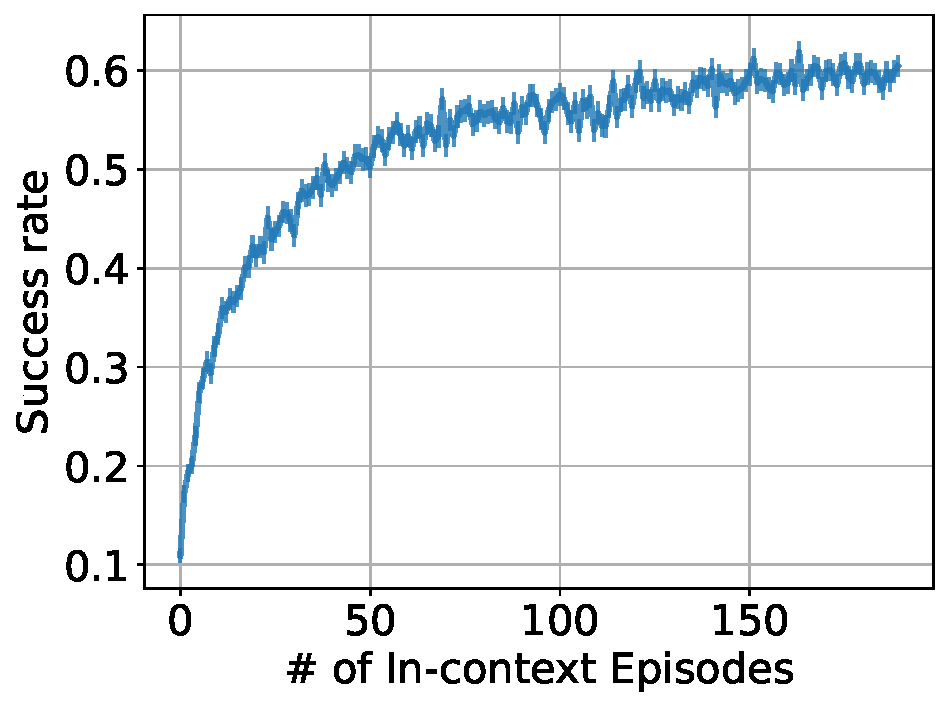
\includegraphics[width=\textwidth]{figures/results/64ksteps_training_inference_custom_pddl_task_success.pdf}
    \caption{Success Rate}
  \end{subfigure}
  \begin{subfigure}[t]{0.45\columnwidth}
    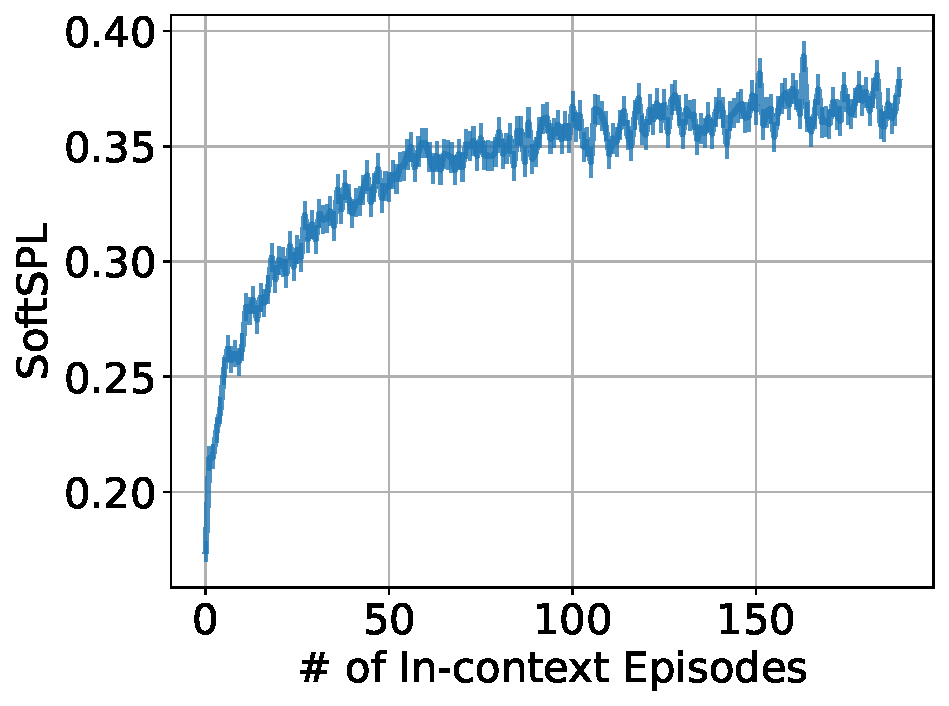
\includegraphics[width=\textwidth]{figures/results/64ksteps_training_inference_spl_geodisc.pdf}
    \caption{Efficiency}
  \end{subfigure}
  \caption{
    The success and efficiency of training and evaluating \method with 64k context length.
  }
  \label{fig:app-64k-training}
\end{figure*}


\begin{figure*}[t]
  \centering
  \begin{subfigure}[t]{0.45\columnwidth}
    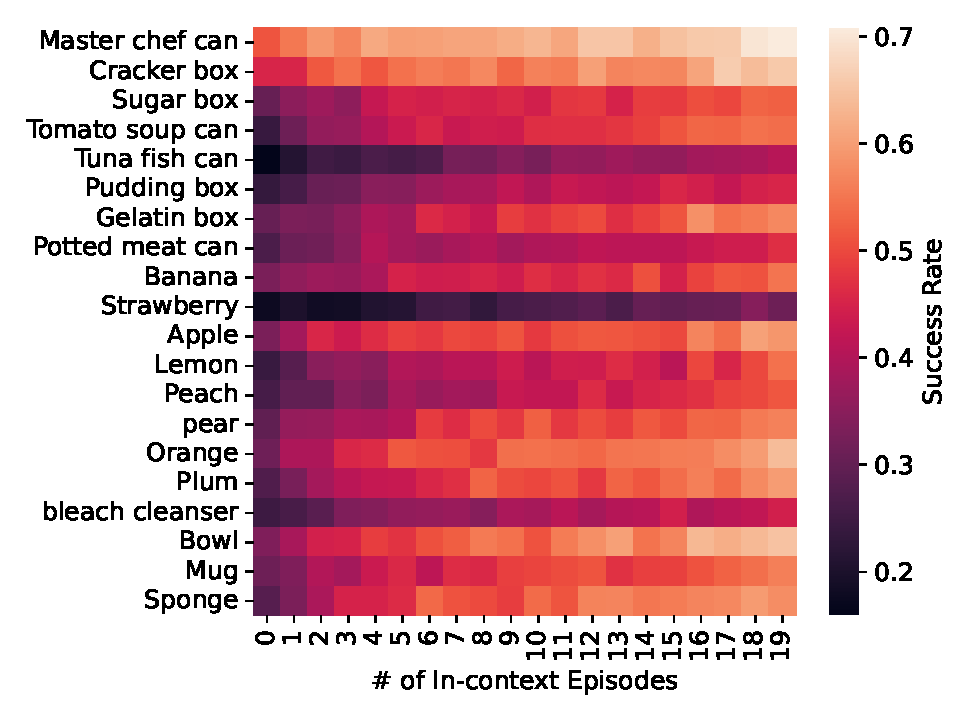
\includegraphics[width=\textwidth]{figures/results/heatmap_epsnum_vs_obj_fixobj_dcm.pdf}
    \caption{Fixed Object Type Per Trial}
    \label{fig:obj-analysis} 
  \end{subfigure}
  \begin{subfigure}[t]{0.45\columnwidth}
    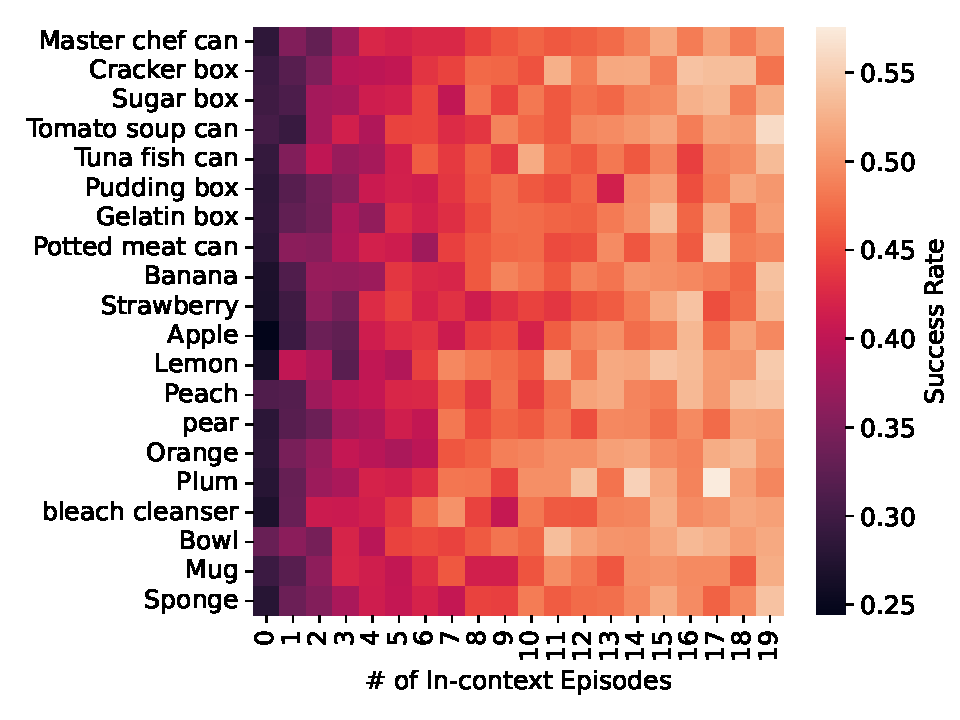
\includegraphics[width=\textwidth]{figures/results/heatmap_epsnum_vs_obj_dcm.pdf}
    \caption{\method per Object Type}
    \label{fig:obj-first-analysis} 
  \end{subfigure}
  \caption{
    Analysis of how \method learns to navigate to particular object types through ICL. 
    (a) compares the number of consecutive episodes within a trial an object appears v.s. the success rate. The agent becomes more capable at navigating to that object type for subsequent episodes. 
    (b) shows the episode index within the trial that the object first appears v.s. the average success rate for different objects. As the agent acquires more experience in-context, it can proficiently navigate to any object type.
  }
  \label{fig:att}
\end{figure*}

\subsection{Analyzing Attention Scores}
\label{sec:app-what-agent-see} 

\begin{figure*}[t!]
  \centering
  \begin{subfigure}[t]{0.24\columnwidth}
    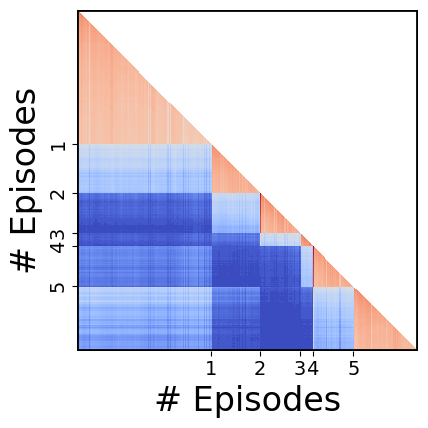
\includegraphics[height=\textwidth]{figures/results/intra-episode-attention.png}
    \caption{Intra-episode attn}
    \label{fig:attn_score_within_eps} 
  \end{subfigure}
  \begin{subfigure}[t]{0.24\columnwidth}
    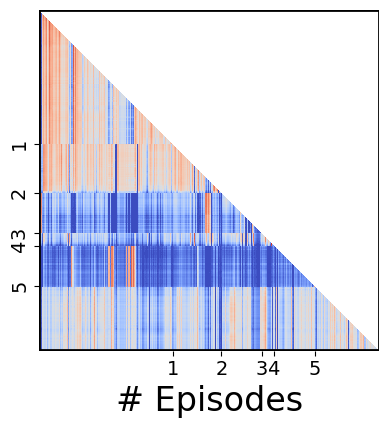
\includegraphics[height=\textwidth]{figures/results/inter-episode-attention.png}
    \caption{Inter-episodes attn}
    \label{fig:attn_score_iea} 
  \end{subfigure}
  \begin{subfigure}[t]{0.24\columnwidth}
    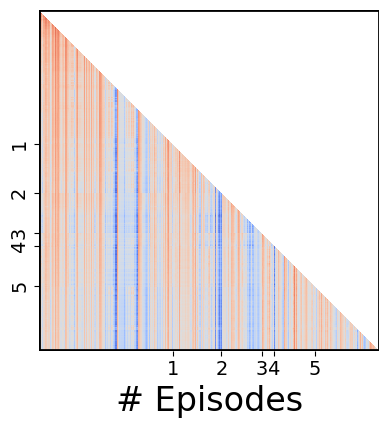
\includegraphics[height=\textwidth]{figures/results/episode-invariant-attention.png}
    \caption{Episode-invariant attn}
    \label{fig:attn_score_eps_invariant} 
  \end{subfigure}
  \begin{subfigure}[t]{0.24\columnwidth}
    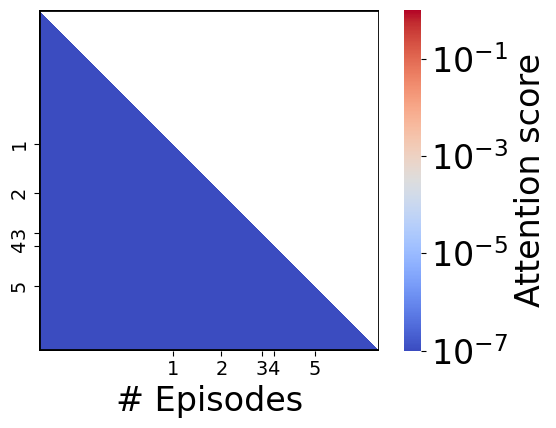
\includegraphics[height=\textwidth]{figures/results/zeros-attention.png}
    \caption{Zero attn}
    \label{fig:attn_score_0} 
  \end{subfigure}
  \vspace{-5pt}
  \caption{
    Attention scores patterns of a sequence with 1024 steps. We found 4 attention patterns in the heads of a trained policy: (a) Intra-episode attention where the attention head assigns high score to the running episode, (b) Inter-episode attention pattern where the attention head assigns high score to the context, without being constrained to the running episode, (c) the episode-invariant pattern where the attention head attends to the same tokens regardless of the episode structure in the context, and (d) the zero attention pattern where the attention head assign all attention scores to the \sinkv.
  }
  \vspace{-15pt}
  \label{fig:attn_score_patts}
\end{figure*}

In this section, we show that the agent is able to utilize the in-context information by inspecting the attention scores patterns in the attention heads. We generate the data by letting the agent interact with an unseen environment for 19 episodes which produced a sequence of 2455 steps. A random object type is selected as a target in each episode. By inspecting the attention scores of the attention heads, we found 4 patterns shown in \Cref{fig:attn_score_patts}. 

\begin{itemize}[itemsep=2pt,topsep=0pt,parsep=0pt,partopsep=0pt,parsep=0pt,leftmargin=*]
  \item \textbf{Intra-episode attention}: In this pattern, the agent attends only to the running episode, \Cref{fig:attn_score_within_eps}.
  \item \textbf{Inter-episodes
attention}: Inter-episodes attention is where the agent accesses the information from previous episodes, \Cref{fig:attn_score_iea}.
  \item \textbf{Episode-invariant attention}: The agent is able to attend to certain tokens which do not change on changing the episode, \Cref{fig:attn_score_eps_invariant}. 
  \item \textbf{Zero attention}: Some heads have 0 attention scores for all tokens which would not be possible with the vanilla attention.
\end{itemize}


We further analyze the attention pattern between successful and failure episodes. We collect 2455 steps in a trial and then probe the agent's attention scores by querying each object type by adding a new observation with the desired object type at the final step. \Cref{fig:trajectory_object_attn_4s} shows that the agent is able to recall multiple instances of the target object types in its history.


\Cref{fig:app_trajectory_object_attn_4s} shows the attention scores for all 20 object types when selected in the 1st step of a new episode after 19 episodes.



\subsection{Impact of Episode Shuffling}
\label{sec:shuffle-abl} 
We ran \method on ReplicaCAD with and without in-context episodes shuffling. \Cref{fig:shuff} shows that \method marginally suffers at in-context learning (ICL) when not shuffling episodes in the context during training. Specifically, the final ICL performance has a 3\% lower success rate and the ICL is less efficient. We believe that shuffling the episodes in the context during the training acts as regularization since it creates diverse contexts.


\begin{figure*}[t]
  \centering
    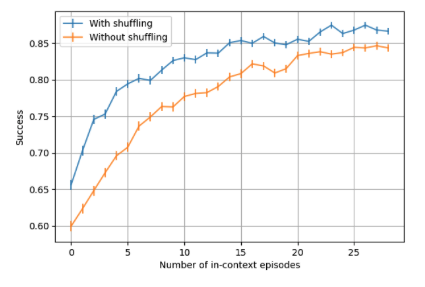
\includegraphics[width=0.5\textwidth]{figures/results/shuffle.png}
    \caption{The effect of shuffling in-context episodes during the training}
  \label{fig:shuff}
\end{figure*}

\subsection{Ablations in Miniworld and Darkroom}
\label{sec:miniworld_abls} 
\begin{figure*}
  \centering
  \begin{subfigure}[t]{0.45\columnwidth}
    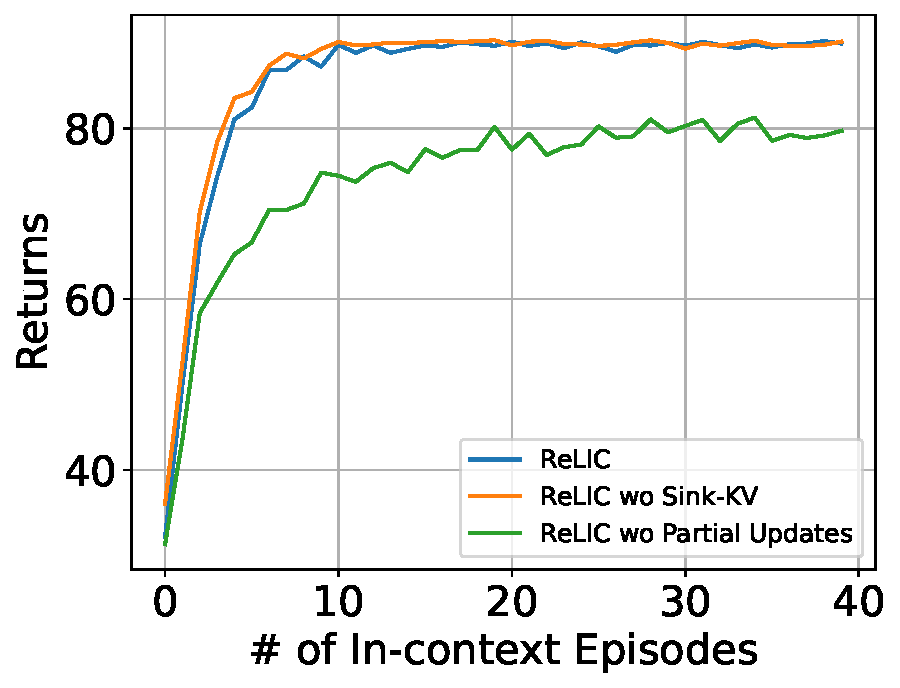
\includegraphics[width=\textwidth]{figures/results/darkroom_ablation.pdf}
    \caption{Darkroom}
    \label{fig:dark_ablation}
  \end{subfigure}
  \begin{subfigure}[t]{0.45\columnwidth}
    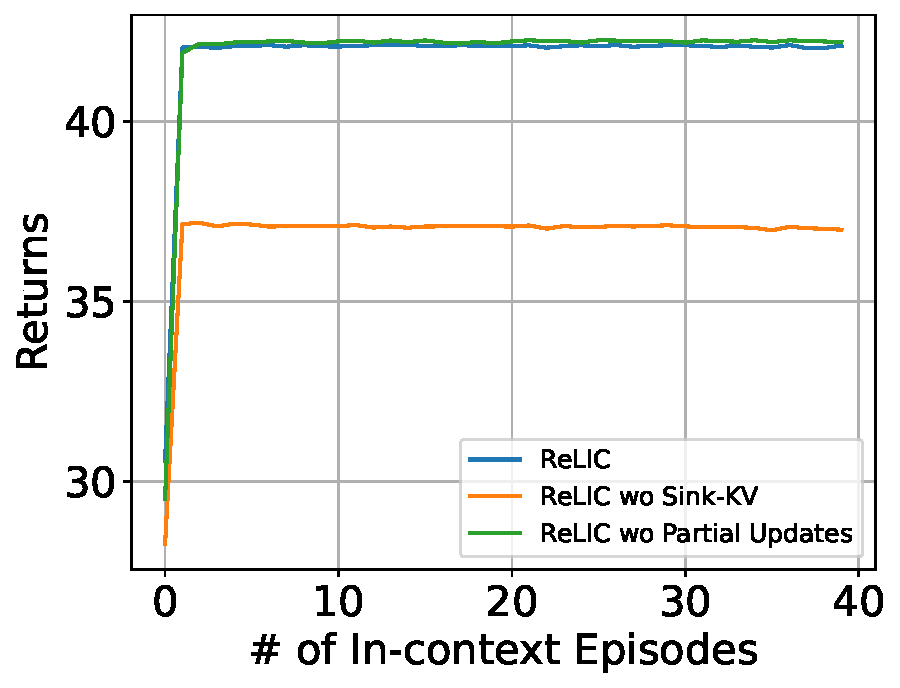
\includegraphics[width=\textwidth]{figures/results/miniworld_ablation.pdf}
    \caption{Miniworld}
    \label{fig:mini_ablation}
  \end{subfigure}
  \caption{
    Ablating \method components on Darkroom and Miniworld.} 
  \label{fig:dark_n_mini_ablation}
\end{figure*}

In this section, we run the partial udpate and \sinkv ablations from \Cref{sec:ablation} on the Darkroom and Miniworld tasks from \Cref{sec:darkroom}. 
The result shows that different components in \method is crucial for different tasks while using \method is as good as or better than \method without its components. The ablation shows that Partial Updates is crucial for long horizon tasks like Darkroom and \task as shown in \cref{fig:dark_ablation,fig:updates}, which have horizon of 100 and 500 steps respectively, but not important for short horizon tasks like Miniworld, which is 50 steps, as shown in \cref{fig:mini_ablation}. It also shows that \sinkv is important for tasks with rich observations like Miniworld and \task, which are visual tasks, compared to the Darkroom, which is a grid world task.


\subsection{Training with 64k Context Length}
\label{sec:app-64k-train-eval}

In the main experiment, we showed that we can train on 4k steps and inference for 32k steps. In this experiment, we show that our method \method is able to train with 64k sequence length. We used the same hyperparameters in the main experiment, except the training sequence length which we set to 64k and the number of updates per rollout is increased so that we do updates every 256 steps, same as the main experiment. 
The result in \Cref{fig:app-64k-training} shows that the model is able to learn and generalize on 64k sequence length.


